
SDL practitioners need to decide which technique, and with what
degree of intensity to use in a particular setting of data release. 
In general the approach to this problem is to employ risk-utility formulations. We assume
below that each candidate method $M(D)$ applied to a dataset $D$ can be characterized by a quantified
\textit{disclosure risk} $\DR (M)$ and \textit{data utility} $\DU
(M)$.  Examples of $\DU(M)$ metrics are given in Section \ref{du_metrics}.
The particular released data, $\DBREL = M(D)$, can be selected from
the candidates in one of two ways. The first is to maximize
utility subject to an upper bound on risk, by solving an
optimization problem of the form
\begin{equation}\label{eq.opt}
\begin{array}{l}
M(D) = {\arg\max}_{M \in \MS} \DU (M) \\[1ex]
\mbox{s.t. } \DR(M) \leq \alpha
\end{array}
\end{equation}
where \MS\ is the set of all possible methods. 

The second and more flexible approach is to define \textit{risk-utility
frontiers} using the partial order $\preceq_{\mathrm{RU}}$ defined
by
\begin{equation}\label{eq.rupo}
M_1 \preceq_{\mathrm{RU}} M_2 \Leftrightarrow \DR(M_2) \leq
\DR(M_1) \qquad\mbox{and}\qquad \DU(M_2) \geq \DU(M_1).
\end{equation}

When $M_1 \preceq_{\mathrm{RU}} M_2$, method $M_2$ is preferred to
$M_1$ because it has both lower disclosure risk and higher
utility. Only candidate releases on the risk-utility frontier of
maximal elements of \RS\ with respect to the partial order
(\ref{eq.rupo}) need be considered further: for any other
candidate, some element of the frontier has lower risk
\textit{and} higher utility. 

Assuming that valid metrics exist for $\DR()$ and $\DU()$, calculation of the frontier can be
done using existing algorithms for finding the maxima in a set of
vectors \citep{kung-luccio-preparata75}. 
The choice among the SDL methods lying on the risk-utility
frontier lies with the data disseminator. To illustrate the first approach
described above, consider Figure \ref{fig.ruplot}, where each point
represents some SDL method characterized in terms of Utility and Risk 
measured according to certain metrics on the horizontal and vertical axes respectively.
If the risk threshold were $10\%$ (in some settings, not a very conservative value), 
then a method denoted as \NOI\ would be the preferred SDL. It is also clear from Figure \ref{fig.ruplot} that compared to \MICZ\ or \NOI\, \MICI\ produces only a minor increase
in utility at an enormous cost in terms of disclosure risk. Similarly,
\RANK\ yields only a modest improvement in disclosure
risk over \MICP\ and \NOI\, but incurs an immense
penalty in terms of data utility. Thus, in a scenario represented by Figure \ref{fig.ruplot}
 the disseminator  might prefer \NOI\ or \MICP\ .

\begin{figure}
\begin{center}
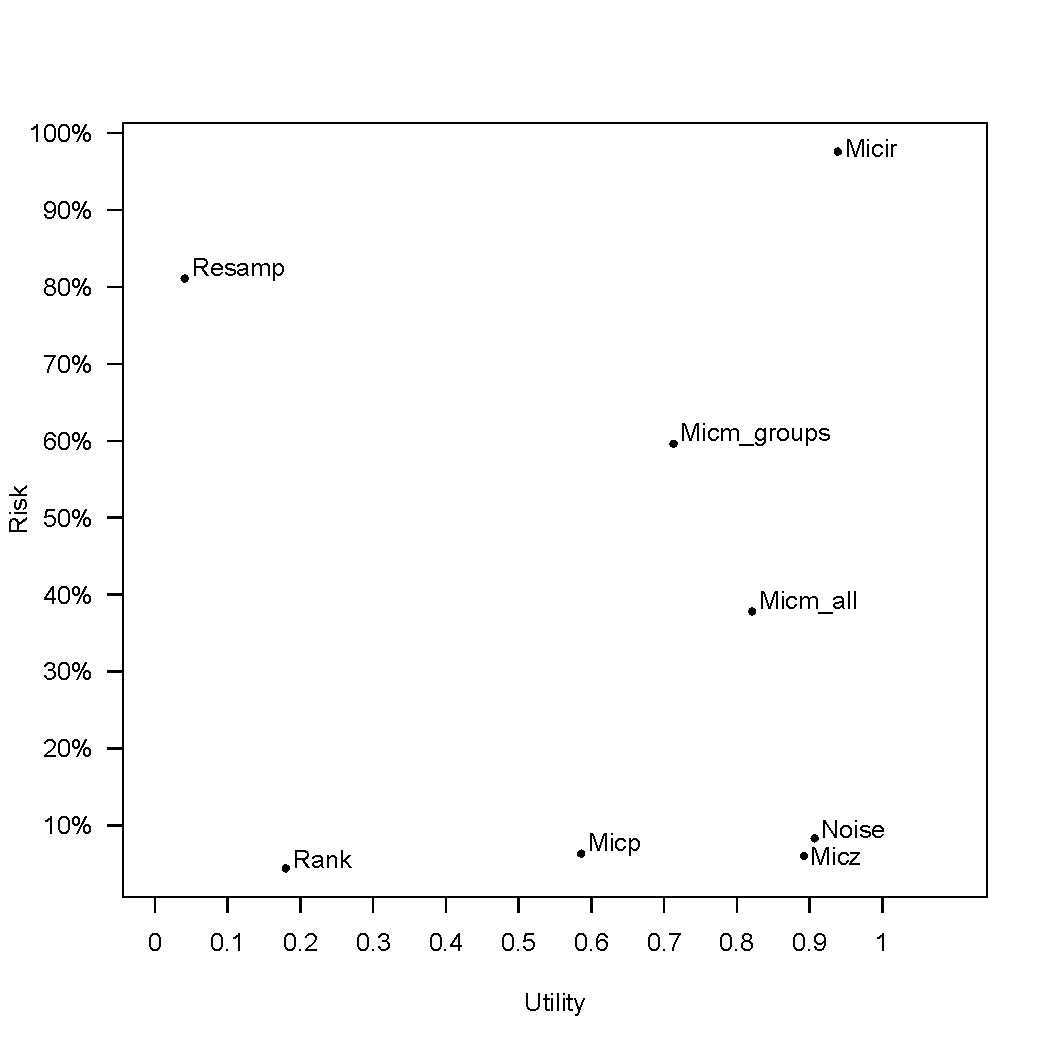
\includegraphics[width=4in]{R_U_plot.pdf}
\end{center}
\caption{Risk-Utility plot}
\label{fig.ruplot}
\end{figure}

